% ================================== HEADER ====================================
\documentclass{article}           % Sets style/look of many things.
% \documentclass{report}          % part, chapters, front page etc.
\usepackage{exsheets}
\usepackage[utf8]{inputenc}       % Encoding of input files UTF-8
\usepackage[T1]{fontenc}
\usepackage[scaled]{beramono}     % Font
\usepackage{color}                % Color text
\usepackage{titlesec}             % Select alternative section titles
\usepackage{fancyvrb}
\usepackage{verbatim}             % Comment environment
\usepackage{listings}             % Format and render text/code etc.
\usepackage{minted}               % Much better syntax highlighting
\usepackage{float}                % Control of floating environment/figure
\usepackage{graphicx,  subfigure} % Better figures, graphics, units etc.
\usepackage{multicol}             % Multiple columns
\usepackage{amsmath}              % Math: Equation, split, align etc.
\usepackage{siunitx}              % SI units
\usepackage{mathtools}            % Different math tools to use with amsmath
\usepackage{amssymb}              % Math symbols
\usepackage[
    colorlinks,
    citecolor=black,              % I like links with standard black color
    filecolor=black,
    linkcolor=black,
    urlcolor=black
]{hyperref}                       % Links in TOC etc.
\usepackage[all]{hypcap}          % Better links to floating environment

\usepackage{tabto}
\newcommand\marginsymbol[1][0pt]{%
  \tabto*{0cm}\makebox[\dimexpr-1cm-#1\relax][r]{$\mathbb{P}$}\tabto*{\TabPrevPos}}

\renewcommand{\thesubsection}{\thesection.\alph{subsection}}
\title{\vspace{-2cm}INF3490/INF4490 Exercises - Week 6}
\author{Eivind Samuelsen, Ole Herman S. Elgesem}
\date{\today}

% Removing paragraph indents is sometimes useful:
\setlength\parindent{0pt}

% Make margins smaller to fit more figures, tables etc on page: (optional)
\addtolength{\oddsidemargin}{-1.0in}
\addtolength{\evensidemargin}{-1.0in}
\addtolength{\textwidth}{2.0in}
\addtolength{\topmargin}{-0.8in}
\addtolength{\textheight}{1.6in}
% ==============================================================================

% ================================= DOCUMENT ===================================
\begin{document}
    \renewcommand\marginsymbol[1][0pt]{%
  \tabto*{0cm}\makebox[-1cm][c]{$\mathbb{P}$}\tabto*{\TabPrevPos}}

\maketitle
\(\mathbb{P}\) marks the programming exercises, we strongly recommend using
the python programming language for these. Exercises may be added/changed
after publishing.


\section{Perceptron activation functions}
Last week we used the activation function
\[
g(h) =
\begin{cases}
      1 & h > 0 \\
      0 & h \leq 0
   \end{cases}
\]
Why is this not used with backpropagation?

\section{Hidden layers}
What is the minimum number of hidden neuron layers needed in order to approximate an arbitrary continuous function, and why?

\section{Validation}
Why do we use a validation set?
Describe how the three different cross-validation methods presented in the lecture slides work, and what their advantages and disadvantages are.

\section{Multi Layer Perceptron}
Implement the MLP shown below, and train it to correctly perform the XOR function.

\begin{figure}[H]
\begin{center}
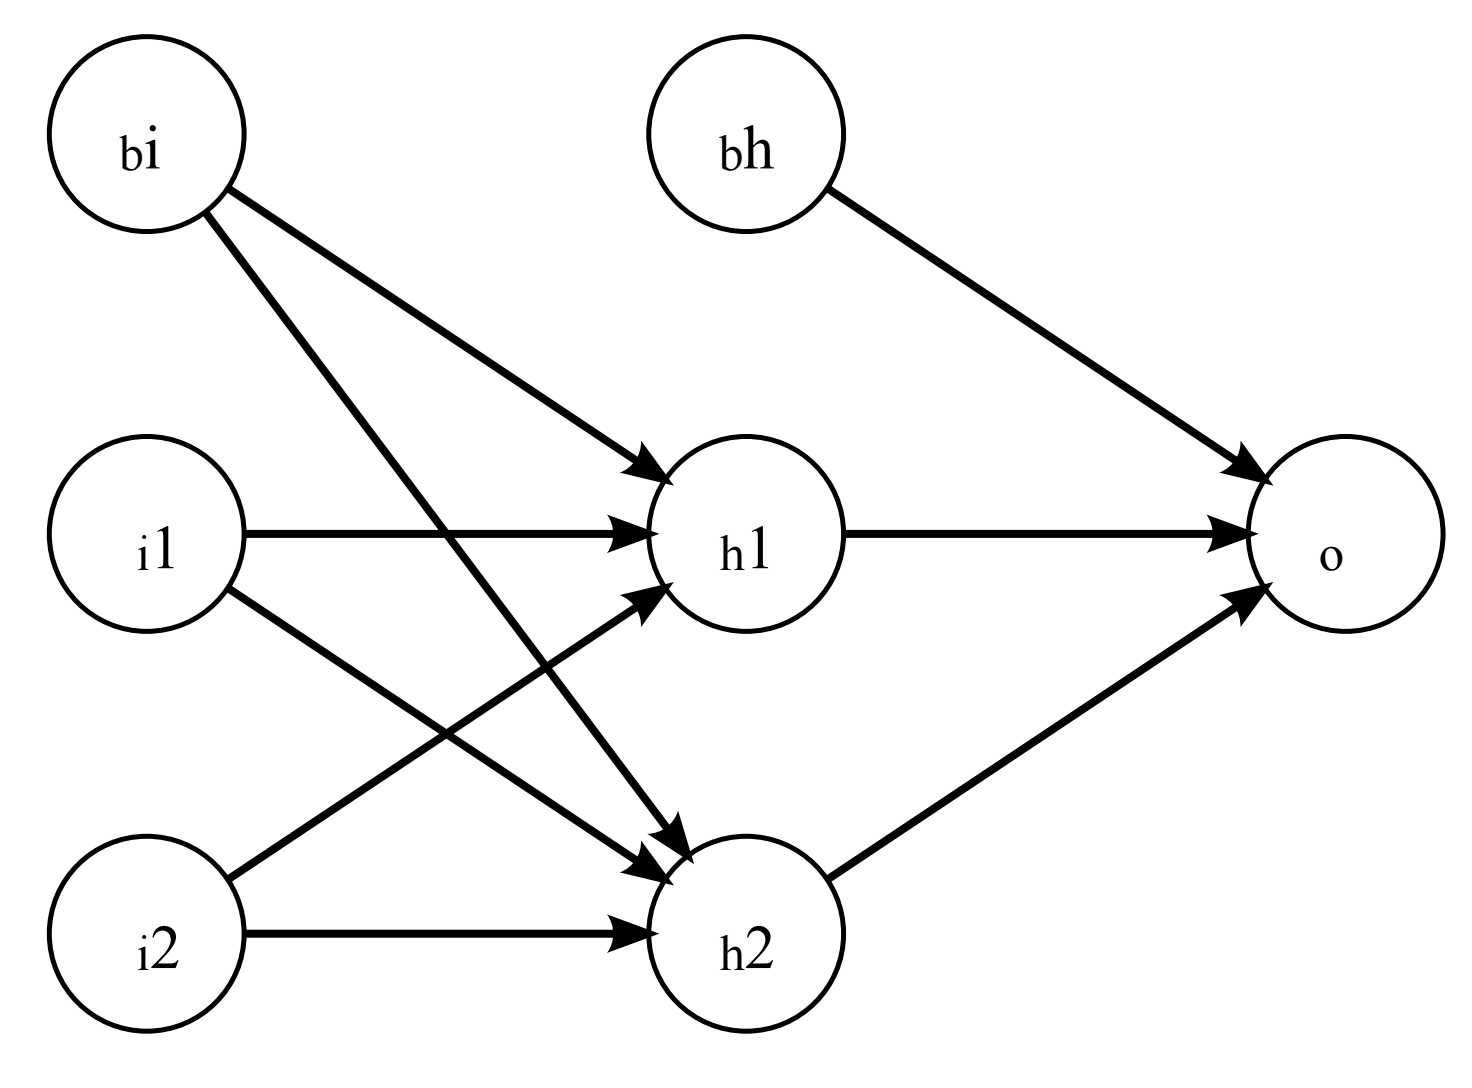
\includegraphics[width=0.4\textwidth]{mlp.png}
\caption{MLP with one hidden layer and two hidden nodes.}
\label{fig:mlp}
\end{center}
\end{figure}

\section{Delta(error) function}
In the lecture slides the backpropagation deltas are first presented as
\[
\delta_k = (y_k - t_k)y_k(1-y_k)
\]
What does this tell us about the activation function in use?

\section{Natural language MLP}
You are to design an MLP that would learn to hyphenate words correctly.
You would have a dictionary that shows correct hyphenation examples for lots of words.
Think about the following:
What should the input to the neural net be?
\begin{itemize}
    \item How should this input be encoded to work well with the classifier?
    \item How is should the output be encoded?
    \item How many layers do you need?
    \item How many neurons should there be in each layer?
\end{itemize}
\section*{Contact and Github}
Corrections of grammar, language, notation or suggestions for improving this material are appreciated.
E-mail me at \href{mailto:olehelg@uio.no}{\textbf{olehelg@uio.no}} or use \href{https://github.com/olehermanse/INF3490-AI_Machine_Learning}{\textbf{GitHub}} to submit an issue or create a pull request.
The \href{https://github.com/olehermanse/INF3490-AI_Machine_Learning}{\textbf{GitHub repository}} contains all source code for assignments, exercises, solutions, examples etc.
As many people have been involved with writing and updating the course material, they are not all listed as authors here.
For a more complete list of authors and contributors see the \href{https://github.com/olehermanse/INF3490-AI_Machine_Learning/blob/master/README.md}{\textbf{README}}.

\end{document}
% ==============================================================================
